\documentclass[10pt]{article}
\usepackage[margin=.74in]{geometry}
\usepackage[T1]{fontenc}
\usepackage{lmodern,microtype,booktabs,graphicx,xcolor,hyperref}
\definecolor{navy}{HTML}{16324F}\definecolor{teal}{HTML}{087E8B}
\hypersetup{colorlinks=true,linkcolor=navy,urlcolor=teal}
\title{\textcolor{navy}{Fresh-Seed Check of the Capacity Control}\\[3pt]
\large An exploratory replication of cluster-conditional adaptation effects}
\author{23I-2581 and 23I-2604\\Data Analysis and Visualization --- Phase 3 research addendum}
\date{18 November 2026}
\begin{document}\maketitle
\begin{abstract}
We reran the corrected matched-capacity protocol with ten evaluation seeds absent from the original diversity/capacity seed banks. This independent-seed sensitivity reproduces the direction of the main task pattern: cluster-conditional models are modestly worse than global refitting on the linear task and better on XOR and five-region tasks. Local experts and the pooled interaction control remain nearly indistinguishable in mean accuracy. Ten seeds provide lower precision; these estimates are exploratory and are not pooled with the 30-seed primary run.
\end{abstract}
\section{Protocol and independence}
The run uses the same locked generator, historical split, 96-batch stream, batch size, frozen three-cluster mapping, four update clocks, feedback delays 0/5/20, shared released-row windows and 8,000-row cumulative repeated-use cap as the corrected 30-seed experiment. Only the evaluation seed bank changes (73116401--73116410). The seed audit scanned 3,097 text files and 4,248 archive metadata members and found no exact seed collisions. Comparisons remain paired within seed. The seed is the bootstrap unit; rows below average outcomes within each seed over four mechanisms and three delays. This narrow follow-up is a sensitivity check, not an adequately powered confirmatory replication.
\section{Results}
\begin{figure}[ht]
\centering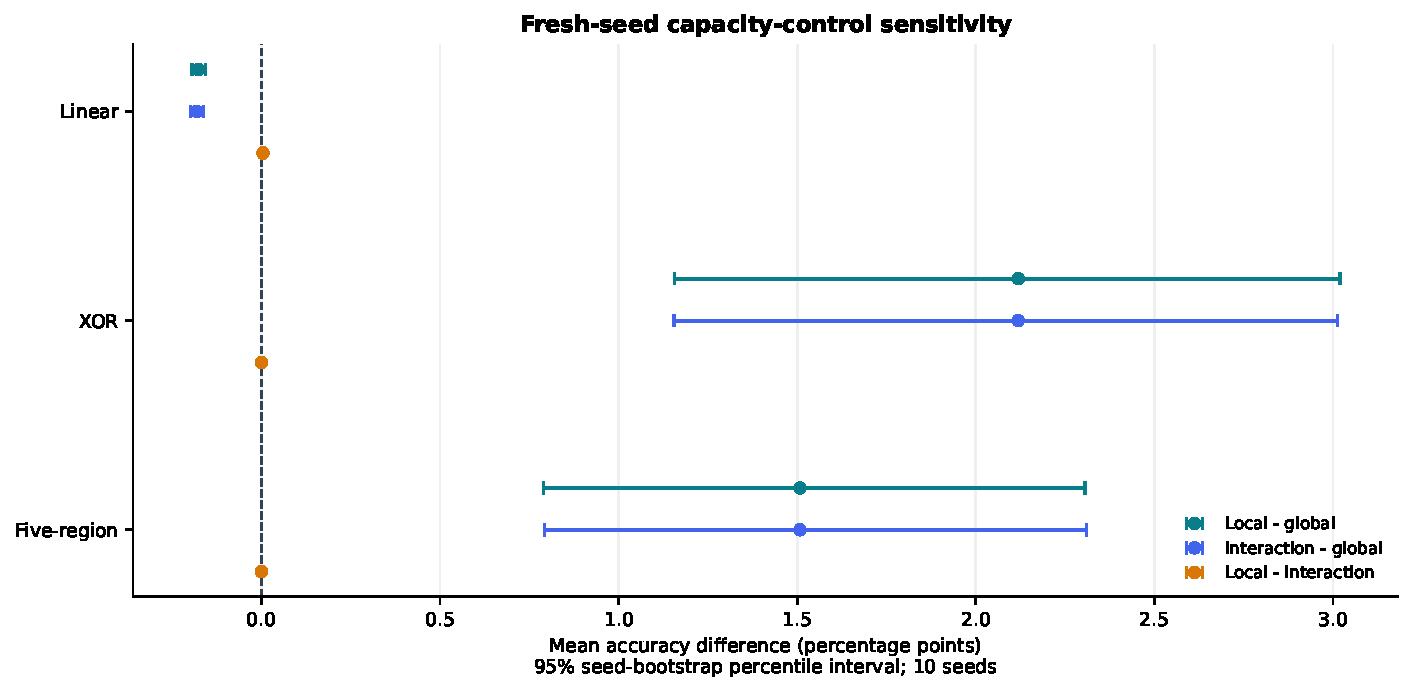
\includegraphics[width=.96\linewidth]{independent_seed_effects.pdf}
\caption{Fresh-seed paired accuracy differences, averaged across mechanisms and delays. Bars show percentile bootstrap intervals over ten seeds. Positive values favor the left-hand model.}
\end{figure}
\begin{table}[ht]
\centering\small\begin{tabular}{@{}lrrr@{}}\toprule
Task & Local $-$ global & Interaction $-$ global & Local $-$ interaction\\\midrule
Linear & -0.18 [-0.19, -0.16] & -0.18 [-0.20, -0.16] & +0.004 [+0.001, +0.009] \\
XOR & +2.12 [+1.16, +3.02] & +2.12 [+1.16, +3.01] & +0.000 [-0.001, +0.002] \\
Five-region & +1.51 [+0.79, +2.31] & +1.51 [+0.79, +2.31] & +0.000 [-0.001, +0.001] \\\bottomrule\end{tabular}
\caption{Mean differences in percentage points with 95\% seed-bootstrap percentile intervals. Four mechanisms and three delays are averaged within each seed before resampling.}
\end{table}
\section{Interpretation and limitations}
The independent seeds reproduce the main qualitative pattern: local and interaction differences from global refitting are negative on linear data and positive on XOR and five-region data. Local-minus-interaction differences are near zero. This supports the capacity/representation interpretation as a pattern worth investigating. The 10-seed intervals are much less stable than the 30-seed analysis, are not multiplicity-adjusted across task contrasts, and should not be treated as independent real-world datasets. Both runs remain synthetic and use one logistic classifier and one fixed cluster count. No claim about causal mechanism, drift-monitoring benefit, natural-domain transfer or analyst benefit follows.
\section{Reproduction}
Reproduce this sensitivity with {\small\url{scripts/reproduce_adaptation_capacity_confirmation.ps1}}. The separate config and run receipt preserve the 10-seed results; do not overwrite the locked 30-seed study.
\end{document}
